\documentclass[10pt,twocolumn]{article}
\usepackage[T1]{fontenc}
\usepackage{newtxtext,newtxmath}
\usepackage[margin=0.75in,columnsep=0.28in]{geometry}
\usepackage[numbers,sort&compress]{natbib}
\usepackage{booktabs,graphicx,xcolor,microtype,amsmath,tabularx,array,url}
\usepackage[font=small,labelfont=bf]{caption}
\usepackage[shortlabels]{enumitem}
\usepackage{tikz}
\usetikzlibrary{positioning,arrows.meta,calc,fit,backgrounds}
\usepackage[hidelinks]{hyperref}

% generated by experiments/analyze.py - do not edit
\newcommand{\AblRuns}{14}
\newcommand{\AdjPLenient}{89\%}
\newcommand{\AdjPLenientCI}{82--93\%}
\newcommand{\AgreeJK}{86\%}
\newcommand{\AuditDebatable}{5}
\newcommand{\AuditN}{40}
\newcommand{\AuditOverlap}{9}
\newcommand{\AuditValid}{31}
\newcommand{\AuditValidCI}{62--88\%}
\newcommand{\AuditValidPct}{78\%}
\newcommand{\AuditWrong}{4}
\newcommand{\Calls}{17 $\pm$ 2}
\newcommand{\CallsAll}{16 $\pm$ 3}
\newcommand{\CallsAllMean}{16}
\newcommand{\CallsGeneric}{14 $\pm$ 2}
\newcommand{\CallsGenericMean}{14}
\newcommand{\CallsMean}{17}
\newcommand{\CurveGenericLast}{15.0}
\newcommand{\CurveGenericSix}{15.0}
\newcommand{\CurvePersonaLast}{16.0}
\newcommand{\CurvePersonaSix}{14.9}
\newcommand{\DetBaseline}{6.8}
\newcommand{\EvidenceVerified}{86\% $\pm$ 6\%}
\newcommand{\EvidenceVerifiedAll}{86\% $\pm$ 6\%}
\newcommand{\EvidenceVerifiedAllMean}{86\%}
\newcommand{\EvidenceVerifiedGeneric}{86\% $\pm$ 5\%}
\newcommand{\EvidenceVerifiedGenericMean}{86\%}
\newcommand{\EvidenceVerifiedMean}{86\%}
\newcommand{\Findings}{89 $\pm$ 11}
\newcommand{\FindingsAll}{84 $\pm$ 14}
\newcommand{\FindingsAllMean}{84}
\newcommand{\FindingsGeneric}{73 $\pm$ 13}
\newcommand{\FindingsGenericMean}{73}
\newcommand{\FindingsMean}{89}
\newcommand{\GenericOnly}{none}
\newcommand{\JacCross}{0.70 $\pm$ 0.09}
\newcommand{\JacCrossMean}{0.70}
\newcommand{\JacGeneric}{0.66 $\pm$ 0.09}
\newcommand{\JacGenericMean}{0.66}
\newcommand{\JacSame}{0.79 $\pm$ 0.20}
\newcommand{\JacSameMean}{0.79}
\newcommand{\KappaJK}{0.62}
\newcommand{\LabelP}{= 0.005}
\newcommand{\LabelPerms}{20{,}000}
\newcommand{\LabelStat}{0.09}
\newcommand{\LambdaFree}{0.60}
\newcommand{\LambdaFreeGeneric}{0.51}
\newcommand{\LambdaSeeded}{0.50}
\newcommand{\MatchedGenericA}{9.1}
\newcommand{\MatchedGenericB}{11.0}
\newcommand{\MatchedGenericC}{12.4}
\newcommand{\MatchedGenericF}{15.0}
\newcommand{\MatchedPersonaA}{11.1}
\newcommand{\MatchedPersonaB}{13.1}
\newcommand{\MatchedPersonaC}{14.0}
\newcommand{\MatchedPersonaF}{15.0}
\newcommand{\McBAllOut}{20}
\newcommand{\McBTextual}{3}
\newcommand{\McBVisual}{17}
\newcommand{\McCAllOut}{1}
\newcommand{\McCTextual}{1}
\newcommand{\McCVisual}{0}
\newcommand{\McPAllOut}{< 0.001}
\newcommand{\McPTextual}{= 0.625}
\newcommand{\McPVisual}{< 0.001}
\newcommand{\Minutes}{5.6 $\pm$ 0.7}
\newcommand{\MinutesAll}{5.3 $\pm$ 0.9}
\newcommand{\MinutesAllMean}{5.3}
\newcommand{\MinutesGeneric}{4.7 $\pm$ 0.9}
\newcommand{\MinutesGenericMean}{4.7}
\newcommand{\MinutesMean}{5.6}
\newcommand{\NGenericRuns}{6}
\newcommand{\NHat}{16.0}
\newcommand{\NHatGeneric}{15.0}
\newcommand{\NPersonaRuns}{12}
\newcommand{\NRuns}{18}
\newcommand{\NeverFound}{U7}
\newcommand{\NoVisAllOut}{82\% $\pm$ 5\%}
\newcommand{\NoVisAllOutMean}{82\%}
\newcommand{\NoVisTextual}{96\% $\pm$ 5\%}
\newcommand{\NoVisTextualMean}{96\%}
\newcommand{\NoVisVisual}{0\% $\pm$ 0\%}
\newcommand{\NoVisVisualMean}{0\%}
\newcommand{\OrigRerunAgree}{95\%}
\newcommand{\OrigRerunKappa}{0.72}
\newcommand{\OrigRerunRecallA}{90\% $\pm$ 5\%}
\newcommand{\OrigRerunRecallAMean}{90\%}
\newcommand{\OrigRerunRecallB}{92\% $\pm$ 4\%}
\newcommand{\OrigRerunRecallBMean}{92\%}
\newcommand{\OrigRerunRuns}{14}
\newcommand{\OutRecall}{90\% $\pm$ 5\%}
\newcommand{\OutRecallAll}{91\% $\pm$ 5\%}
\newcommand{\OutRecallAllMean}{91\%}
\newcommand{\OutRecallGeneric}{94\% $\pm$ 5\%}
\newcommand{\OutRecallGenericMean}{94\%}
\newcommand{\OutRecallMean}{90\%}
\newcommand{\PLenient}{98\% $\pm$ 2\%}
\newcommand{\PLenientAll}{98\% $\pm$ 2\%}
\newcommand{\PLenientAllMean}{98\%}
\newcommand{\PLenientGeneric}{99\% $\pm$ 1\%}
\newcommand{\PLenientGenericMean}{99\%}
\newcommand{\PLenientMean}{98\%}
\newcommand{\PStrict}{53\% $\pm$ 6\%}
\newcommand{\PStrictAll}{55\% $\pm$ 6\%}
\newcommand{\PStrictAllMean}{55\%}
\newcommand{\PStrictGeneric}{59\% $\pm$ 4\%}
\newcommand{\PStrictGenericMean}{59\%}
\newcommand{\PStrictMean}{53\%}
\newcommand{\PersonaOnly}{U17}
\newcommand{\PooledDuplicate}{405}
\newcommand{\PooledFindings}{1{,}504}
\newcommand{\PooledIncorrect}{24}
\newcommand{\PooledMatched}{418}
\newcommand{\PooledPLenient}{98\%}
\newcommand{\PooledPStrict}{55\%}
\newcommand{\PooledUnseeded}{657}
\newcommand{\PvGOutDiff}{$-4$}
\newcommand{\PvGOutP}{= 0.177}
\newcommand{\PvGPStrictDiff}{$-6$}
\newcommand{\PvGPStrictP}{= 0.049}
\newcommand{\PvGUXDiff}{$+11$}
\newcommand{\PvGUXExpDiff}{$+10$}
\newcommand{\PvGUXExpP}{= 0.023}
\newcommand{\PvGUXP}{= 0.028}
\newcommand{\RetestAgree}{94\%}
\newcommand{\RetestKappa}{0.57}
\newcommand{\RetestRecallA}{92\% $\pm$ 4\%}
\newcommand{\RetestRecallAMean}{92\%}
\newcommand{\RetestRecallB}{93\% $\pm$ 5\%}
\newcommand{\RetestRecallBMean}{93\%}
\newcommand{\RetestRuns}{14}
\newcommand{\RmseFree}{0.90}
\newcommand{\RmseSeeded}{1.56}
\newcommand{\SignLAllOut}{0}
\newcommand{\SignLTextual}{1}
\newcommand{\SignLVisual}{0}
\newcommand{\SignPAllOut}{< 0.001}
\newcommand{\SignPTextual}{= 0.625}
\newcommand{\SignPVisual}{< 0.001}
\newcommand{\SignWAllOut}{13}
\newcommand{\SignWTextual}{3}
\newcommand{\SignWVisual}{14}
\newcommand{\Steps}{13.5 $\pm$ 2.1}
\newcommand{\StepsAll}{12.9 $\pm$ 2.0}
\newcommand{\StepsAllMean}{12.9}
\newcommand{\StepsGeneric}{11.7 $\pm$ 1.2}
\newcommand{\StepsGenericMean}{11.7}
\newcommand{\StepsMean}{13.5}
\newcommand{\SusBusyParentMobile}{48.8}
\newcommand{\SusEslParent}{21.2}
\newcommand{\SusGenericUser}{42.5}
\newcommand{\SusGrandparentStorykeeper}{37.5}
\newcommand{\SusLowVisionSenior}{38.8}
\newcommand{\SusPrivacyConsciousParent}{40.0}
\newcommand{\SusTechSavvyParent}{38.8}
\newcommand{\UXRecall}{65\% $\pm$ 8\%}
\newcommand{\UXRecallAll}{61\% $\pm$ 10\%}
\newcommand{\UXRecallAllMean}{61\%}
\newcommand{\UXRecallExp}{67\% $\pm$ 8\%}
\newcommand{\UXRecallExpAll}{63\% $\pm$ 9\%}
\newcommand{\UXRecallExpAllMean}{63\%}
\newcommand{\UXRecallExpGeneric}{57\% $\pm$ 9\%}
\newcommand{\UXRecallExpGenericMean}{57\%}
\newcommand{\UXRecallExpMean}{67\%}
\newcommand{\UXRecallGeneric}{54\% $\pm$ 10\%}
\newcommand{\UXRecallGenericMean}{54\%}
\newcommand{\UXRecallMean}{65\%}
\newcommand{\UnionOut}{14}
\newcommand{\UnionUX}{16}
\newcommand{\UnseededShare}{44\%}
\newcommand{\VisAllOut}{92\% $\pm$ 4\%}
\newcommand{\VisAllOutMean}{92\%}
\newcommand{\VisTextual}{97\% $\pm$ 4\%}
\newcommand{\VisTextualMean}{97\%}
\newcommand{\VisVisual}{61\% $\pm$ 21\%}
\newcommand{\VisVisualMean}{61\%}


\newcommand{\sys}{\textsf{userqa}}
\newcommand{\site}{StoryHearth}
\newcommand{\ol}{\textsf{ourlegacy.family}}
\newcolumntype{Y}{>{\raggedright\arraybackslash}X}
\newcolumntype{P}[1]{>{\raggedright\arraybackslash}p{#1}}
\setlist{nosep,leftmargin=*}
\raggedbottom
\setlength{\textfloatsep}{10pt plus 2pt minus 3pt}
\setlength{\floatsep}{8pt plus 2pt minus 2pt}
\setlength{\dbltextfloatsep}{10pt plus 2pt minus 3pt}

\title{Simulated Users Who Read the Output:\\Persona-Grounded LLM Agents for Usability and Output Evaluation of Generative Websites}
\author{Anonymous authors\thanks{Code, personas, the \site{} benchmark and every run record (traces, LLM calls, assessments, scores) are in the accompanying repository.}}
\date{September 2026}

\begin{document}
\maketitle

\begin{abstract}
Websites that generate personalised artefacts, such as picture books written from a family's memories, can fail their users in two places: on the way through the interface, and in what the generator produces. User studies catch both but are slow and costly, and the LLM-based simulated users proposed so far stop at the interface. We present \sys{}, an open-source agent that plays a specified kind of user on a live website. It reviews every screen it reaches, carries out the site's main task, and then critiques every part of what the site generated (page text, pictures and downloaded files), proposing a concrete change and rewritten text for each part. Personas operationalise constructs from HCI (goal-directed personas, GenderMag cognitive facets, Big Five traits, Westin privacy segments, CEFR language levels), and the browser environment enforces device, skimming and low-vision constraints instead of merely describing them. We evaluate the agent, driven by a free model through OpenRouter, on \site{}, a synthetic storybook site it has never seen, with 17 seeded usability defects and 14 seeded output defects. Across \NRuns{} sessions, persona-conditioned sessions found \UXRecallMean{} of the usability defects against \UXRecallGenericMean{} for a no-persona agent (exact permutation $p \PvGUXP$), at lower strict precision (\PStrictMean{} vs \PStrictGenericMean{}). Output recall was high in both conditions (\OutRecallMean{} vs \OutRecallGenericMean{}), and together the sessions found \UnionUX{} of 17 usability defects and all 14 output defects. Withholding the pictures from the output critic removed every detection of the picture-only defects (\VisVisualMean{} to \NoVisVisualMean{}). On the real site \ol{}, the agent signed up with a disposable inbox, made a book, returned to repair it, and documented how the product rewrote the family's relationships. The same case study exposed five failure modes of the evaluator itself, all attribution errors, which we analyse and fix.
\end{abstract}

\section{Introduction}
\label{sec:intro}

A growing class of consumer websites does not just present content; it generates content for each user. On a personalised storybook site, a grandmother types a memory (``the summer my father made me a kite out of an old blue shirt''), names her grandson as the hero, picks an illustration style, and receives a book. Such products can fail in two places. The interface can fail her: a vague call to action, a photo upload that does not say where her grandson's face will be stored, a text box that silently drops the end of her story. And the output can fail her: the book can turn her father into ``Grandpa's daddy'', draw her as a boy, or end mid-sentence. For generative products, the second kind of failure is often the one that matters most, because the output \emph{is} the product.

Usability practice has good instruments for the first kind of failure: think-aloud testing~\cite{ericsson1993protocol}, heuristic evaluation~\cite{nielsen1990heuristic,nielsen1994heuristic} and the cognitive walkthrough~\cite{polson1992cognitive,wharton1994cognitive}. They are costly, and any single evaluator finds only part of the problems: two evaluators' problem sets typically overlap by only 5--65\%~\cite{hertzum2001evaluator}, and in CUE-4 most problems were reported by just one of 17 professional teams~\cite{molich2008cue4}. Evaluating generated output is harder still, because every user gets a different output, and whether it is right depends on what that user asked for.

Two lines of LLM research make a simulated alternative plausible. Web agents can now operate real browsers~\cite{yao2023react,zhou2024webarena,deng2023mind2web,zheng2024seeact,he2024webvoyager,koh2024visualwebarena}, and LLMs can play specified people with some fidelity~\cite{park2023generative,argyle2023out,moon2024virtual,jiang2024personallm}. Simulated usability testing has started to combine the two~\cite{lu2025uxagent,xiang2024simuser}, but existing systems evaluate the interface only and rarely measure what their simulated users find against a known ground truth. It is also unclear whether the persona matters at all, or whether a persona is a label that produces stereotyped behaviour~\cite{cheng2023compost,wang2025large}.

We present \sys{}, a persona-grounded agent for both halves of the problem. Our design rests on five ideas:
\begin{enumerate}[(i)]
\item \textbf{A persona is a mechanism, not a label.} Personas specify goals and frustrations, GenderMag cognitive facets~\cite{burnett2016gendermag}, Big Five traits, attitudes and language level, and these are turned into behavioural rules.
\item \textbf{Perception is enforced by the environment.} A phone user sees a phone viewport, a skimming user sees truncated paragraphs, and a low-vision user cannot read text that fails contrast checks.
\item \textbf{Findings are inspection-grade.} Every new screen gets a structured review with walkthrough questions, heuristic codes, a severity, quoted evidence (checked against the page) and a proposed fix.
\item \textbf{The output is read part by part, in the persona's frame.} Every page and picture gets a reaction, rubric problems, a concrete change and, where the text should change, a rewrite.
\item \textbf{Attribution is explicit.} The critic is told which words came from the user, which edits superseded which, and what the user entered on earlier visits, so that it blames the site only for what the site did.
\end{enumerate}

We evaluate \sys{} on \site{}, a synthetic storybook site that the agent has never seen, with 31 seeded defects, and on the live product \ol{}. Our contributions are:
\begin{itemize}
\item the design and an open implementation of a persona-grounded agent that evaluates both a website's usability and its generated output, safely enough to run on production sites with free models (\S\ref{sec:system});
\item an output-critique method that attributes content to the user or the site across edits, regenerated versions and repeat visits (\S\ref{sec:output});
\item \site{}, a benchmark with 17 seeded usability and 14 seeded output defects, and a scoring protocol that combines an LLM judge, a keyword baseline, exposure-adjusted recall and an audit of the judge's decisions (\S\ref{sec:benchmark}--\ref{sec:setup});
\item an empirical study (\S\ref{sec:results}). Persona conditioning raises usability recall and changes which defects are found; pictures are necessary for picture defects; and a live case study yields five evaluator failure modes, each with its fix and a before-and-after comparison (\S\ref{sec:case}).
\end{itemize}

\section{Related work}
\label{sec:related}

\paragraph{Usability evaluation.} Heuristic evaluation asks evaluators to judge an interface against principles such as visibility of system status and error prevention~\cite{nielsen1990heuristic,nielsen1994heuristic}. The cognitive walkthrough asks, for each action, whether users will try to achieve the right effect, notice the control, associate it with the effect, and see progress~\cite{polson1992cognitive,wharton1994cognitive}. Concurrent think-aloud gives access to users' reasoning~\cite{ericsson1993protocol}. The evaluator effect~\cite{hertzum2001evaluator,molich2008cue4} and problem-discovery models~\cite{nielsen1993mathematical,virzi1992refining} explain why several evaluators or participants are needed: in Nielsen and Landauer's model, each participant finds a share $\lambda$ of the problems, $0.31$ on average across their projects. Standard post-session instruments include SUS~\cite{brooke1996sus,bangor2009determining,sauro2016quantifying}, UEQ-S~\cite{schrepp2017ueqs} and likelihood to recommend~\cite{reichheld2003one}. Dark-pattern research catalogues deceptive designs such as pre-ticked add-ons, hidden costs and false urgency~\cite{gray2018dark,mathur2019dark}. We reuse these instruments inside the agent's prompts and record their outputs.

\paragraph{Personas.} Goal-directed personas~\cite{cooper1999inmates,pruitt2003personas} describe users by goals, context and frustrations. GenderMag~\cite{burnett2016gendermag} replaced demographic descriptions with five cognitive facets (motivation, information processing style, computer self-efficacy, attitude to risk and learning style) that predict how people approach software. We also draw on the Big Five~\cite{john1999big}, technology acceptance~\cite{davis1989perceived}, Westin's privacy segments~\cite{kumaraguru2005privacy}, CEFR language levels~\cite{coe2001cefr} and WCAG~\cite{w3c2023wcag,w3c2017stories}.

\paragraph{Web agents.} ReAct interleaves reasoning and acting~\cite{yao2023react}. WebArena gives agents a numbered accessibility tree of realistic sites~\cite{zhou2024webarena}. Mind2Web, SeeAct, WebVoyager and VisualWebArena extend web agents to real websites and screenshots~\cite{deng2023mind2web,zheng2024seeact,he2024webvoyager,koh2024visualwebarena}. These systems optimise task success; we use the same machinery to model a particular user's experience, including the moments where that user would struggle.

\paragraph{LLMs as simulated people.} Generative agents keep a memory stream to behave coherently over time~\cite{park2023generative}. LLM ``silicon samples'' reproduce some survey response patterns of human subgroups~\cite{argyle2023out} and can replicate classic experiments, sometimes with hyper-accurate distortions~\cite{aher2023using}. LLMs can also generate plausible HCI research data~\cite{hamalainen2023evaluating}. Backstories~\cite{moon2024virtual} and explicit trait prompts~\cite{jiang2024personallm,serapio2023personality} make personas more consistent, and role play is a useful frame for what such agents do~\cite{shanahan2023role}. There are serious caveats. LLM opinions are skewed toward some groups~\cite{santurkar2023whose}, simulations drift into caricature~\cite{cheng2023compost}, identity-based prompting misportrays and flattens groups~\cite{wang2025large}, and replacing participants risks an illusion of inclusion~\cite{agnew2024illusion}. Synthetic survey data is also less varied and less stable than human data~\cite{bisbee2024synthetic}, and LLM survey answers show non-human response biases~\cite{tjuatja2024llms,dominguez2024questioning}. These caveats shaped our design: we use facet-based personas, audit the simulation for caricature and knowledge leakage, and treat self-reports with suspicion.

\paragraph{LLM-based usability evaluation.} UXAgent runs persona-conditioned LLM agents on web designs and produces both behavioural data and interviews~\cite{lu2025uxagent}. SimUser simulates diverse users of mobile apps to generate usability feedback~\cite{xiang2024simuser}. Duan et al.\ generate heuristic feedback on UI mockups~\cite{duan2024generating}, and AXNav replays accessibility tests from natural language~\cite{taeb2024axnav}. None of these critiques the content a site generates, and none reports recall against seeded ground truth with a no-persona ablation.

\paragraph{LLM judges.} Rubric-based LLM evaluation with evidence before scores~\cite{liu2023geval,kim2024prometheus} correlates with human judgement but is prone to biases~\cite{zheng2023judging} and sycophancy~\cite{sharma2024sycophancy}. Our output critic is such a judge, placed in the persona's frame, and it also proposes changes, much as self-critique proposes revisions in Self-Refine~\cite{madaan2023selfrefine}.

\section{System}
\label{sec:system}

\subsection{Overview and design goals}
\label{sec:overview}

Figure~\ref{fig:arch} shows the pipeline. A \emph{persona} and a \emph{site configuration} define a session. The site configuration gives the URL, the task in the words a study participant would be given, the allowed domains, credentials or a disposable inbox, a spend rule and budgets. The \emph{persona agent} makes one LLM call per step. It receives the persona-filtered observation from the \emph{browser environment}, thinks aloud, reviews any new screen, and returns a batch of actions. After the session, the \emph{output assessor} critiques everything the site generated, a \emph{debrief} administers questionnaires and an interview, and a \emph{fidelity audit} rates how faithfully the persona was played. Everything is written to a report and to machine-readable records.

Six goals guided the design: \textbf{G1} behaviour follows persona mechanisms rather than labels; \textbf{G2} the agent perceives only what that person would; \textbf{G3} findings carry evidence that can be checked; \textbf{G4} every generated part is critiqued with a proposed fix; \textbf{G5} content is attributed correctly to the user or the site; \textbf{G6} sessions are safe, cheap and fully logged, so that they can run on production sites with free models and be re-scored later without new browsing.

\begin{figure*}[t]
\centering
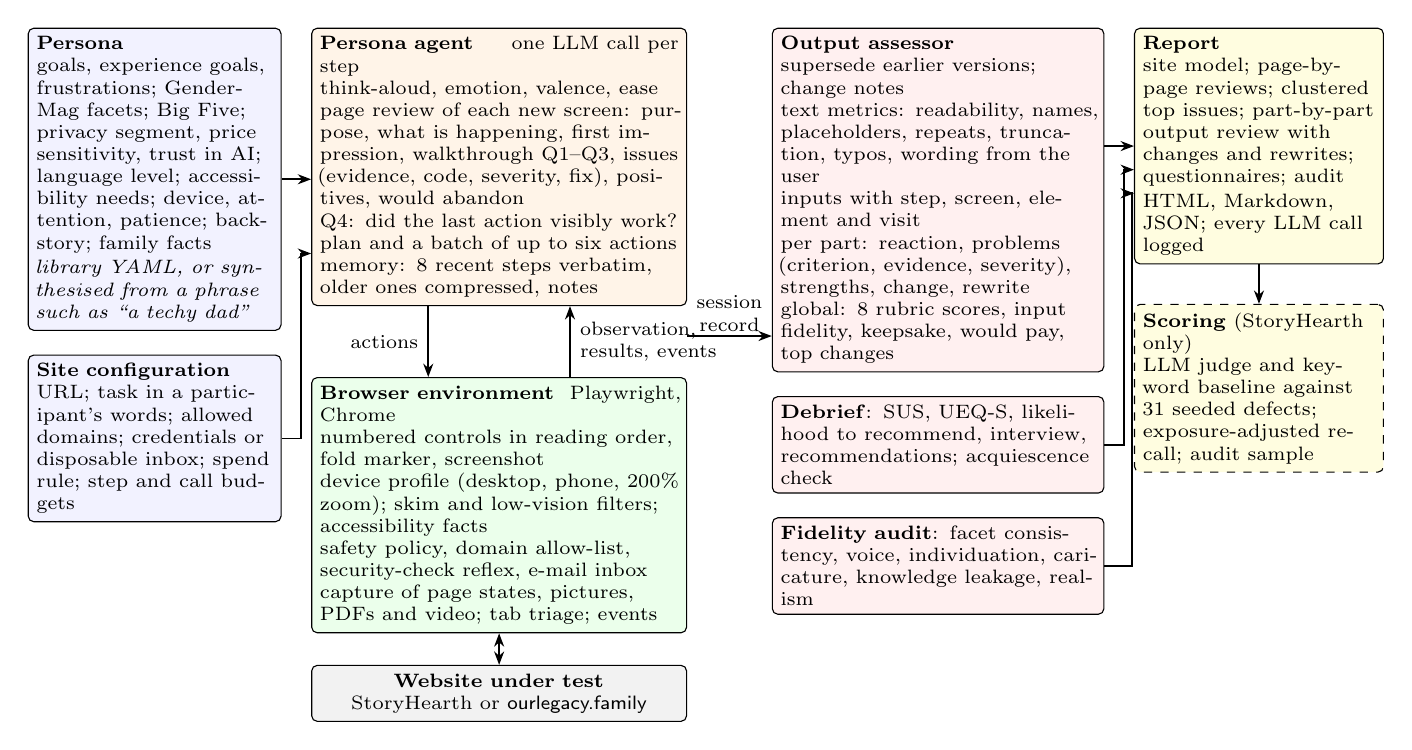
\begin{tikzpicture}[font=\scriptsize,
  box/.style={draw, rounded corners=2pt, inner sep=3pt, align=left},
  arr/.style={-{Stealth[length=1.7mm]}, semithick}]
\node[box, fill=blue!5, text width=3.0cm, anchor=north west] (persona) at (0,0) {\textbf{Persona}\\goals, experience goals, frustrations; GenderMag facets; Big Five; privacy segment, price sensitivity, trust in AI; language level; accessibility needs; device, attention, patience; backstory; family facts\\[1pt]\emph{library YAML, or synthesised from a phrase such as ``a techy dad''}};
\node[box, fill=blue!5, text width=3.0cm, below=3mm of persona.south west, anchor=north west] (siteconf) {\textbf{Site configuration}\\URL; task in a participant's words; allowed domains; credentials or disposable inbox; spend rule; step and call budgets};
\node[box, fill=orange!9, text width=4.55cm, anchor=north west] (agent) at (3.6,0) {\textbf{Persona agent}\hfill one LLM call per step\\think-aloud, emotion, valence, ease\\page review of each new screen: purpose, what is happening, first impression, walkthrough Q1--Q3, issues (evidence, code, severity, fix), positives, would abandon\\Q4: did the last action visibly work?\\plan and a batch of up to six actions\\memory: 8 recent steps verbatim, older ones compressed, notes};
\node[box, fill=green!8, text width=4.55cm, below=9mm of agent.south west, anchor=north west] (env) {\textbf{Browser environment}\hfill Playwright, Chrome\\numbered controls in reading order, fold marker, screenshot\\device profile (desktop, phone, 200\% zoom); skim and low-vision filters; accessibility facts\\safety policy, domain allow-list, security-check reflex, e-mail inbox\\capture of page states, pictures, PDFs and video; tab triage; events};
\node[box, fill=gray!10, text width=4.55cm, below=4mm of env.south west, anchor=north west, align=center] (web) {\textbf{Website under test}\\\site{} or \ol{}};
\draw[arr] ([xshift=-9mm]agent.south) -- node[left] {actions} ([xshift=-9mm]env.north);
\draw[arr] ([xshift=9mm]env.north) -- node[right, align=left] {observation,\\results, events} ([xshift=9mm]agent.south);
\draw[arr, {Stealth[length=1.7mm]}-{Stealth[length=1.7mm]}] (env.south) -- (web.north);
\draw[arr] (persona.east) -- (agent.west |- persona.east);
\draw[arr] (siteconf.east) -- ++(0.25,0) |- ([yshift=-11mm]agent.west);
\node[box, fill=red!6, text width=4.0cm, anchor=north west] (assess) at (9.45,0) {\textbf{Output assessor}\\supersede earlier versions; change notes\\text metrics: readability, names, placeholders, repeats, truncation, typos, wording from the user\\inputs with step, screen, element and visit\\per part: reaction, problems (criterion, evidence, severity), strengths, change, rewrite\\global: 8 rubric scores, input fidelity, keepsake, would pay, top changes};
\node[box, fill=red!6, text width=4.0cm, below=3mm of assess.south west, anchor=north west] (debrief) {\textbf{Debrief}: SUS, UEQ-S, likelihood to recommend, interview, recommendations; acquiescence check};
\node[box, fill=red!6, text width=4.0cm, below=3mm of debrief.south west, anchor=north west] (audit) {\textbf{Fidelity audit}: facet consistency, voice, individuation, caricature, knowledge leakage, realism};
\node[box, fill=yellow!12, text width=2.95cm, anchor=north west] (report) at (14.05,0) {\textbf{Report}\\site model; page-by-page reviews; clustered top issues; part-by-part output review with changes and rewrites; questionnaires; audit\\[1pt]HTML, Markdown, JSON; every LLM call logged};
\node[box, fill=yellow!12, text width=2.95cm, draw, dashed, below=5mm of report.south west, anchor=north west] (score) {\textbf{Scoring} (\site{} only)\\LLM judge and keyword baseline against 31 seeded defects; exposure-adjusted recall; audit sample};
\coordinate (mid) at ($(agent.east)!0.5!(env.east)$);
\draw[arr] (mid) -- node[above, align=center, inner sep=1.5pt] {session\\record} (assess.west |- mid);
\draw[arr] (assess.east |- report.west) -- (report.west);
\draw[arr] (debrief.east) -- ++(0.25,0) |- ([yshift=-3mm]report.west);
\draw[arr] (audit.east) -- ++(0.35,0) |- ([yshift=-6mm]report.west);
\draw[arr] (report.south) -- (score.north);
\end{tikzpicture}
\caption{Architecture of \sys{}. The persona agent and the browser environment alternate for up to a step budget; the post-session stages read the session record (trace, page reviews, inputs, captures, waits and abandonment), and every stage can be re-run on a finished session without browsing again.}
\label{fig:arch}
\end{figure*}

\subsection{Personas}
\label{sec:personas}

A persona (Appendix~\ref{app:personas}) has a name, age and occupation; a first-person backstory, following the Anthology approach~\cite{moon2024virtual}; end goals, experience goals and frustrations~\cite{cooper1999inmates,pruitt2003personas}; the five GenderMag facets~\cite{burnett2016gendermag}; Big Five descriptors~\cite{john1999big}; attitudes (Westin privacy segment~\cite{kumaraguru2005privacy}, price sensitivity, trust in AI); a language level such as CEFR B1~\cite{coe2001cefr}; accessibility needs; a device; an attention mode; a patience in steps; and concrete domain facts. The domain facts include the child who should be the hero, the other character, the memory to tell, a treasured object, a place and a reading age. These facts are what the persona types when the site asks, so the output can be checked against them.

Facets become behavioural rules in the system prompt. A low self-efficacy persona ``never types web addresses by hand, never guesses hidden features, and describes things in everyday words'' and tends to blame itself; a selective information processor ``acts on the first promising cue''; a risk-averse persona avoids clicking things whose consequences are unclear. All personas are told to scan for words that match their goal (information scent~\cite{pirolli1999information}), to take the first option that looks right (satisficing~\cite{simon1956rational}), and to ``notice what a person like you would notice, and miss what you would miss''. A persona can also be synthesised from a phrase such as ``a family-oriented grandparent'' by an LLM call that fills in the same schema. The \emph{generic} baseline replaces the whole profile with ``You are a typical adult web user (no further persona details)'' followed by the domain facts; it keeps the same task, environment and instruments.

\subsection{Browser environment}
\label{sec:env}

The environment wraps Playwright~\cite{playwright} around a headed Chrome, since headless browsers attract more bot challenges. Its observation follows WebArena~\cite{zhou2024webarena}: the page text in reading order, with every interactive element numbered and described by role, accessible name and state, plus a marker where the viewport ends (``fold'') and, optionally, a screenshot. A screen state is identified by its path, first heading and any open dialog, so that each state of a single-page app gets its own review.

\paragraph{Perception.} Device profiles set the viewport: desktop (1280$\times$800), phone (390$\times$844, touch, mobile user agent) or 200\% zoom (640$\times$400 at device scale factor 2). The attention filter works in the page script. \emph{Skim} cuts every text block longer than 14 words to its first 10 words and an ellipsis. \emph{Low vision} replaces text whose contrast ratio is below 3:1, or whose size is below 11\,px, with a marker saying the persona cannot make it out, and blurs the screenshot. The same script computes WCAG facts~\cite{w3c2023wcag}: contrast failures, text below 12\,px, targets smaller than 24\,px that fail the WCAG 2.2 spacing exception, and controls without an accessible name. A low-vision persona is told about these in perceptual terms (``some controls are tiny and hard for you to hit: [6], [7]''), and a phone persona is reminded that it taps with its thumb. The filters stop a persona from reading what its real counterpart could not, but the notes also encode our assumptions about what such users perceive (\S\ref{sec:limitations}).

\paragraph{Actions.} The actions are click, type, select, set\_range, upload, scroll, press, go\_back, wait\_for\_change (until the page changes, for long generations), read\_inbox (for e-mailed codes), read\_page (full text on the next step), flip\_through (page through a multi-page result and capture every page), done and give\_up. Each result is reported in plain words. A \texttt{type} result, for example, says when the field kept fewer characters than were typed, as a person watching the text appear would see it stop.

\paragraph{Safety.} Clicks on controls matching pay, buy, purchase, place order, subscribe, upgrade, buy credits, add card or delete account are hard-blocked, and so is typing into payment-card and banking fields. Controls showing a price are soft-blocked unless the site configuration allows them; for \ol{}, the generate buttons were allowed because a new account's free credits pay for them. Navigation is restricted to allowed domains plus sign-in providers. Tokens, codes and signatures are redacted from logged URLs and console errors.

\paragraph{Reflexes and captures.} Some things a person does without thinking, and the environment does them too, reporting each one to the agent as an \emph{event}. It ticks ``Verify you are human'' checkboxes~\cite{turnstile}: at most three clicks, up to 12\,s to resolve, every outcome logged, and never a script inside the challenge frame or any attempt at image or puzzle CAPTCHAs. It triages new tabs. When the site hands over a PDF, image or video, it opens the file and reads every page or frame, reporting, for example, ``The site gave you a PDF \ldots; you opened it and looked through all 32 pages''. Output captures record the page text, crops of every picture with its alt text, and viewport screenshots.

\subsection{Agent loop and page reviews}
\label{sec:agent}

Each step is one LLM call, which fits free-tier budgets. The call fuses three instruments. The first is concurrent think-aloud in the persona's voice~\cite{ericsson1993protocol}, with an emotion from a fixed list, a valence ($-2$..$2$) and an ease rating (1--7). The second is a \emph{page review} whenever the screen state is new: its purpose; an objective account of what is happening; a first impression, as in a five-second test; walkthrough questions Q1--Q3 for the next action~\cite{wharton1994cognitive}; issues; positives; and whether the persona would abandon here. After each action, Q4 asks whether the site clearly showed that the action worked. Each issue has a title, exact evidence (a quote or an element number), a code, a severity for this persona (0--4)~\cite{nielsen1994heuristic}, why it matters to the persona, and a concrete fix. The codes are H1--H10~\cite{nielsen1994heuristic} plus ACC, TRUST, VALUE, DECEPTIVE and CONTENT. The third instrument is a ReAct-style plan~\cite{yao2023react} with up to six actions; anything that loads a new screen ends the batch. On the first step the agent also writes a \emph{site model}: what the site is, who it is for, its value proposition, main tasks, pricing and trust signals, and whether it fits the persona.

An episodic memory, after the memory stream of \citet{park2023generative}, replays the last eight steps verbatim (thought, actions, result) and compresses older ones to a line; explicit notes such as a price or a code are always kept. Quoted evidence is checked against the page text; an issue counts as \emph{verified} when every quotation in its evidence occurs on the page. An abandonment model records the first self-reported abandonment, or the step at which consecutive frustrating steps (valence $\le -1$, a failed action, or a screen that has stopped changing) exceed the persona's patience. In the experiments the session then continues (``note'' mode), so that the rest of the journey is still evaluated. Issues are clustered by token overlap within a code family for the report.

\subsection{Output assessment}
\label{sec:output}

\paragraph{Capture and versions.} The agent flags generated content when it sees it, and the environment captures files. A session can capture the same output many times: while it is still being generated and after it is finished, after the user edits a scene, or as a regenerated PDF. Reviewing every capture as a separate part would duplicate parts and, worse, blame the site for states the user has already fixed. The assessor therefore removes boilerplate (lines on at least 60\% of captures, and pagers), keeps sentence-like lines as prose, and supersedes a capture when a later capture of the same page contains at least 80\% of its prose lines. For files, a later file of the same type and page count supersedes an earlier one when at least 60\% of its pages keep at least 80\% of their lines. Each final version carries a \emph{change note} saying what the persona would notice changed since the first version: lines no longer there, new lines, and pictures redrawn, detected by a 256-bit average hash differing in more than 40 bits. Screenshots of the browser's PDF viewer are dropped when the PDF itself was captured.

\paragraph{Evidence from tools.} Deterministic checks run on the prose: Flesch--Kincaid grade~\cite{kincaid1975derivation} against the requested reading age; mentions of the names the user entered, and near-miss spellings; capitalised names that were not in the inputs; template placeholders; repeated sentences; an abrupt ending; and dictionary misses. A final check lists \emph{wording the output repeats from the user's own inputs} (shared word sequences), so that the critic does not blame the site for the user's own phrases. These measurements are given to the critic as evidence to verify, not as verdicts.

\paragraph{Inputs and provenance.} The critic sees the persona's inputs in order, each tagged with the step, screen and form element it went into. An entry that was later replaced in the same element is marked as superseded, and a cleared field is shown as cleared. On a return visit, the inputs of all earlier visits are carried forward and tagged ``earlier visit''. Element identity is scoped per visit, because element numbers are only stable within one visit and a label alone is ambiguous: every scene's edit box on \ol{} is called ``Narrative Text''. Section~\ref{sec:errors} shows why each of these details was needed; they, and the list of wording repeated from the inputs, were added after the \site{} experiments (\S\ref{sec:setup}).

\paragraph{Critique.} The critic plays the persona but is told to be a careful and fair evaluator. Its rubric has eight criteria with score anchors: fidelity to the user's details, coherence, age fit, language, text--image fit, character consistency, visual quality and emotional resonance. It gives evidence before each score, in the style of G-Eval and Prometheus~\cite{liu2023geval,kim2024prometheus}. For every part in order (cover, title page, each page, each file page) it returns the verbatim text, the pictures it refers to with a description of what they actually show, a reaction in character, problems (criterion, evidence, severity), strengths, the change it would make to this part, and a rewrite when the text should change. Globally it returns the eight scores, an input-fidelity account (used correctly, missing, changed, invented), safety concerns, an overall reaction, keepsake-worthiness (1--5), whether it would pay, and the top changes. Long outputs are reviewed one artefact at a time, in batches of at most 12 pictures, with the parts already reviewed listed so that they are not repeated, followed by a synthesis call that produces the global judgement. Appendix~\ref{app:example} shows two parts from a \site{} session.

\subsection{Questionnaires and fidelity audit}
\label{sec:debrief}

After the output review, the persona answers SUS~\cite{brooke1996sus}, graded on the curved scale of \citet{sauro2016quantifying}, and UEQ-S~\cite{schrepp2017ueqs}. It also rates likelihood to recommend (0--10)~\cite{reichheld2003one}, answers eight interview questions (purpose, worst and best moment, where it would have given up, what was missing, trust, willingness to pay, verdict on the output), and lists the changes it wants most. Because LLM survey answers show non-human response biases~\cite{tjuatja2024llms,dominguez2024questioning}, the persona gives a one-line reason before each SUS rating, SUS keeps its alternating item polarity~\cite{sauro2011positive}, and we flag sessions that agree, or disagree, with both items of two or more positive/negative pairs.

A separate call audits the simulation, not the website, from a transcript of the session. The transcript lists, for each step, what the browser had just reported, the persona's feeling, thought and actions. The audit rates, on 1--5 scales with justifications citing steps, whether behaviour matched each specified facet, voice consistency, individuation and caricature (after CoMPosT~\cite{cheng2023compost}), knowledge leakage (knowledge or skills the person would not have, cf.\ the hyper-accuracy distortion of \citet{aher2023using}), and overall realism. The audit runs at temperature 0 and is skipped for the generic baseline, which has no persona to be faithful to.

\subsection{Implementation and cost}
\label{sec:impl}

\sys{} is about 4,400 lines of Python, plus 1,100 lines of experiment scripts and 88 unit and end-to-end tests. The end-to-end test drives a real browser through a small local site with a scripted LLM. The LLM client talks to OpenRouter~\cite{openrouter}. It enforces a per-session call budget, retries with back-off, falls back to other free models on errors, salvages truncated JSON, and logs every request and response with its purpose (images are replaced by a digest). Step calls use temperature 0.7; the output critic 0.3; the debrief 0.5; the audit and the scoring judge 0. Every post-session stage can be re-run on a finished session (\texttt{reassess}, \texttt{reaudit}), which is how we ran the ablations and applied the fixes of \S\ref{sec:errors} without browsing the live site again.

\section{The StoryHearth benchmark}
\label{sec:benchmark}

\site{} is a synthetic website for personalised illustrated storybooks, written for this study and never shown to the agent. It has nine HTML pages: home, log-in, sign-up, dashboard, a four-step creation wizard, the book viewer, pricing, checkout and a privacy notice. Two scripts implement the wizard and generate the book. The wizard asks for the hero's name, age and pronouns, the other character, the treasured object, the place, the memory itself, an illustration style, a reading level and a photo of the child. After a 15-second wait, the site produces a nine-page book whose text is composed from the user's inputs and whose illustrations are SVG pictures drawn from them, so every persona gets its own book.

We seeded 17 usability defects (Appendix~\ref{app:defects}) and 14 output defects (Table~\ref{tab:output}), chosen to cover Nielsen's heuristics, accessibility, trust, dark patterns and every rubric criterion. The usability defects include a vague ``Proceed~$\to$'' call to action, jargon hero copy, a footer at about 1.4:1 contrast, placeholder-only log-in labels, a cryptic ``Error 0x80070057'' banner, a wizard without a progress indicator, a textarea that silently truncates at 200 characters, reading levels given as Lexile codes, a child-photo upload without privacy information, an unlabelled spinner, 20$\times$20\,px icon-only page-turn buttons, no way to edit a single page, a pre-ticked \pounds7.99 gift wrap, shipping revealed only at checkout, a false-urgency countdown and a currency switch from \$ to \pounds. The output defects include a typo in the title, unfilled placeholders, a misspelled name, a pronoun switch, a missing character, an invented ``Uncle Bartholomew'', the treasured object replaced by ``a shiny red balloon'', ornate vocabulary, a frightening passage, an illustration that shows sunshine while the text says it is pouring, a hair-colour change, a repeated opening sentence, a truncated ending and the wrong illustration style. Two output defects (O10 and O11) are visible only in the pictures, and one (O14) in both text and pictures. The ground truth is stored outside the web root.

\section{Experimental setup}
\label{sec:setup}

\paragraph{Sessions.} We ran six personas (Appendix~\ref{app:personas}): a grandparent storyteller, a tech-savvy parent, a busy parent on a phone who skims, a parent reading English at CEFR B1, a low-vision senior at 200\% zoom, and a privacy-conscious parent. Each ran twice, and the generic baseline ran six times, giving \NRuns{} sessions. All sessions received the same task: log in, create a book about the family memory in the profile, read every page, and find out what a printed hardcover would really cost without paying. Budgets were 32 steps and 45 LLM calls per session, with screenshots sent at every step. Sessions ran three at a time, launched 20\,s apart. A pilot session was excluded.

\paragraph{Code versions.} The \site{} sessions ran before the fixes of \S\ref{sec:errors}: twelve from a frozen snapshot of commit \texttt{dcc3677}, and the first six, which started before the snapshot mechanism existed, from the working tree shortly before that commit. Their output assessor therefore lacked per-artefact batching, change notes, input provenance and the list of wording repeated from the inputs. The re-assessments of \S\ref{sec:vision} and \S\ref{sec:reliability} ran about half an hour later, with per-artefact batching and change notes but still without the attribution fixes. \site{} sessions rarely exercise these features, because the persona enters its story once, in one visit, and never regenerates the book. Still, the \site{} numbers describe these earlier versions, not the system exactly as described in \S\ref{sec:system}.

\paragraph{Model.} All calls used \texttt{stealth/space-bunny-alpha}, a free vision-capable model served by OpenRouter whose provider is not disclosed, with free models as fallbacks. The \NRuns{} sessions made 289 calls, all served by the primary model with no failures: 232 steps, 22 output critiques, 4 syntheses, 18 debriefs and 13 audit calls (12 audits plus one repair). They used 1.48\,M prompt tokens and 0.42\,M completion tokens. The median step call took 9.5\,s (90th percentile 14\,s).

\paragraph{Scoring.} Findings are the agent's formal reports only: page-review issues and later issues (usability), and the output assessment's per-part problems, input-fidelity misses and safety concerns (output). Think-aloud mentions do not count. An LLM judge at temperature 0 matches each finding to at most one seeded defect, strictly (the same element or content \emph{and} the same kind of problem). It classes unmatched findings as \emph{valid but unseeded} or \emph{incorrect}; repeat matches of a defect are duplicates. Strict precision is the share of findings that match a seeded defect, counting duplicates; lenient precision also counts valid-unseeded findings. A transparent keyword baseline (same kind of defect, same page for usability defects, any defect keyword) checks the judge. Recall is reported raw, and \emph{exposure-adjusted} over the defects a session could have met: pages it visited and conditions it triggered, such as typing more than 200 characters. We also record which output defects the deterministic text metrics flag on their own. Because the judge's ``valid'' class is generous, a random sample of \AuditN{} valid-unseeded findings was audited against the site source, the captured text and the screenshots. It had a single annotator, the AI coding assistant that built \site{}, not a person (\S\ref{sec:limitations}).

\paragraph{Ablations and reliability.} For the vision ablation, we re-ran the output assessment of \AblRuns{} sessions (all 12 persona sessions and the first two generic ones) on the \emph{same captured outputs}, once with pictures and once with text and alt text only. A second run with pictures gives test--retest reliability. Because the captures are identical, differences are due to the critic alone.

\paragraph{Statistics.} Persona and generic sessions are compared with exact two-sided permutation tests over all $\binom{18}{6}=18{,}564$ splits. To ask whether the persona determines \emph{which} defects are found, we compare the mean Jaccard similarity of the found usability-defect sets between same-persona and different-persona pairs of the 12 persona sessions, with a one-sided label-permutation test (\LabelPerms{} permutations, $p=(\text{ge}+1)/(\text{perms}+1)$~\cite{phipson2010permutation,good2005permutation}). Paired vision comparisons use exact McNemar tests~\cite{mcnemar1947note} per session and defect, and sign tests over sessions. Agreement is reported as percentage and Cohen's $\kappa$~\cite{cohen1960coefficient}, interpreted after \citet{landis1977measurement}, and proportions carry Wilson intervals~\cite{wilson1927probable}. Discovery curves average 500 random session orders and are fitted with the Nielsen--Landauer model $\mathit{found}(n)=N(1-(1-\lambda)^n)$~\cite{nielsen1993mathematical} by least squares. We report nominal $p$-values without correction for multiple comparisons.

\section{Results}
\label{sec:results}

\begin{table*}[t]
\centering
\small
\setlength{\tabcolsep}{5pt}
\caption{Seeded-defect detection on StoryHearth per persona (mean $\pm$ SD over repetitions; LLM-judge matching). UX (usability) recall over 17 seeded UX defects, raw and over the defects the session was exposed to; output recall over 14 seeded output defects. Strict precision: share of findings matching a seeded defect; lenient additionally counts findings judged valid but unseeded. The generic agent is the no-persona ablation.}
\label{tab:detection}
\begin{tabular}{lccccccccc}
\toprule
Persona & $n$ & \begin{tabular}[b]{@{}c@{}}UX\\recall\end{tabular} & \begin{tabular}[b]{@{}c@{}}UX recall\\(exposed)\end{tabular} & \begin{tabular}[b]{@{}c@{}}Output\\recall\end{tabular} & \begin{tabular}[b]{@{}c@{}}Precision\\(strict)\end{tabular} & \begin{tabular}[b]{@{}c@{}}Precision\\(lenient)\end{tabular} & Findings & \begin{tabular}[b]{@{}c@{}}LLM\\calls\end{tabular} & Minutes \\
\midrule
Grandparent & 2 & 0.74 $\pm$ 0.04 & 0.74 $\pm$ 0.04 & 0.89 $\pm$ 0.05 & 0.62 $\pm$ 0.02 & 0.96 $\pm$ 0.02 & 78 $\pm$ 5 & 15 $\pm$ 1 & 5.3 $\pm$ 1.2 \\
Tech-savvy & 2 & 0.65 $\pm$ 0.08 & 0.67 $\pm$ 0.06 & 0.89 $\pm$ 0.05 & 0.48 $\pm$ 0.02 & 0.99 $\pm$ 0.02 & 100 $\pm$ 6 & 18 $\pm$ 1 & 5.4 $\pm$ 0.5 \\
Busy/mobile & 2 & 0.59 $\pm$ 0.00 & 0.62 $\pm$ 0.00 & 0.89 $\pm$ 0.05 & 0.54 $\pm$ 0.01 & 0.98 $\pm$ 0.02 & 81 $\pm$ 10 & 15 $\pm$ 0 & 5.4 $\pm$ 0.6 \\
ESL & 2 & 0.68 $\pm$ 0.21 & 0.68 $\pm$ 0.21 & 0.93 $\pm$ 0.00 & 0.52 $\pm$ 0.09 & 1.00 $\pm$ 0.00 & 96 $\pm$ 15 & 18 $\pm$ 5 & 6.0 $\pm$ 0.9 \\
Low vision & 2 & 0.65 $\pm$ 0.00 & 0.65 $\pm$ 0.00 & 0.86 $\pm$ 0.10 & 0.55 $\pm$ 0.04 & 0.97 $\pm$ 0.02 & 85 $\pm$ 10 & 17 $\pm$ 1 & 5.5 $\pm$ 0.3 \\
Privacy & 2 & 0.62 $\pm$ 0.04 & 0.66 $\pm$ 0.04 & 0.93 $\pm$ 0.00 & 0.47 $\pm$ 0.00 & 0.99 $\pm$ 0.00 & 94 $\pm$ 1 & 18 $\pm$ 1 & 6.1 $\pm$ 1.0 \\
Generic (ablation) & 6 & 0.54 $\pm$ 0.10 & 0.57 $\pm$ 0.09 & 0.94 $\pm$ 0.05 & 0.59 $\pm$ 0.04 & 0.99 $\pm$ 0.01 & 73 $\pm$ 13 & 14 $\pm$ 2 & 4.7 $\pm$ 0.9 \\
\midrule
\textit{All personas} & 12 & 0.65 $\pm$ 0.08 & 0.67 $\pm$ 0.08 & 0.90 $\pm$ 0.05 & 0.53 $\pm$ 0.06 & 0.98 $\pm$ 0.02 & 89 $\pm$ 11 & 17 $\pm$ 2 & 5.6 $\pm$ 0.7 \\
\bottomrule
\end{tabular}
\end{table*}


\subsection{Detection}
\label{sec:detection}

All \NRuns{} sessions completed the task and reached the generated book, in \StepsAllMean{} steps, \CallsAllMean{} LLM calls and \MinutesAllMean{} minutes on average. Table~\ref{tab:detection} gives detection by persona. Persona sessions found \UXRecall{} of the seeded usability defects, against \UXRecallGeneric{} for the generic agent. The difference of \PvGUXDiff{} percentage points is significant ($p \PvGUXP$) and survives exposure adjustment (\UXRecallExpMean{} vs \UXRecallExpGenericMean{}, \PvGUXExpDiff{} points, $p \PvGUXExpP$). Output recall was high and did not differ significantly (\OutRecallMean{} vs \OutRecallGenericMean{}, $p \PvGOutP$). Persona sessions were also longer (\StepsMean{} vs \StepsGenericMean{} steps) and wrote more findings (\FindingsMean{} vs \FindingsGenericMean{}), and their strict precision was lower (\PStrictMean{} vs \PStrictGenericMean{}, \PvGPStrictDiff{} points, $p \PvGPStrictP$): personas report more, including more problems outside the seeded set. Lenient precision was \PLenientMean{} and \PLenientGenericMean{}. Of the findings with quoted evidence, \EvidenceVerifiedMean{} had every quotation verified on the page.

\begin{figure*}[t]
\centering
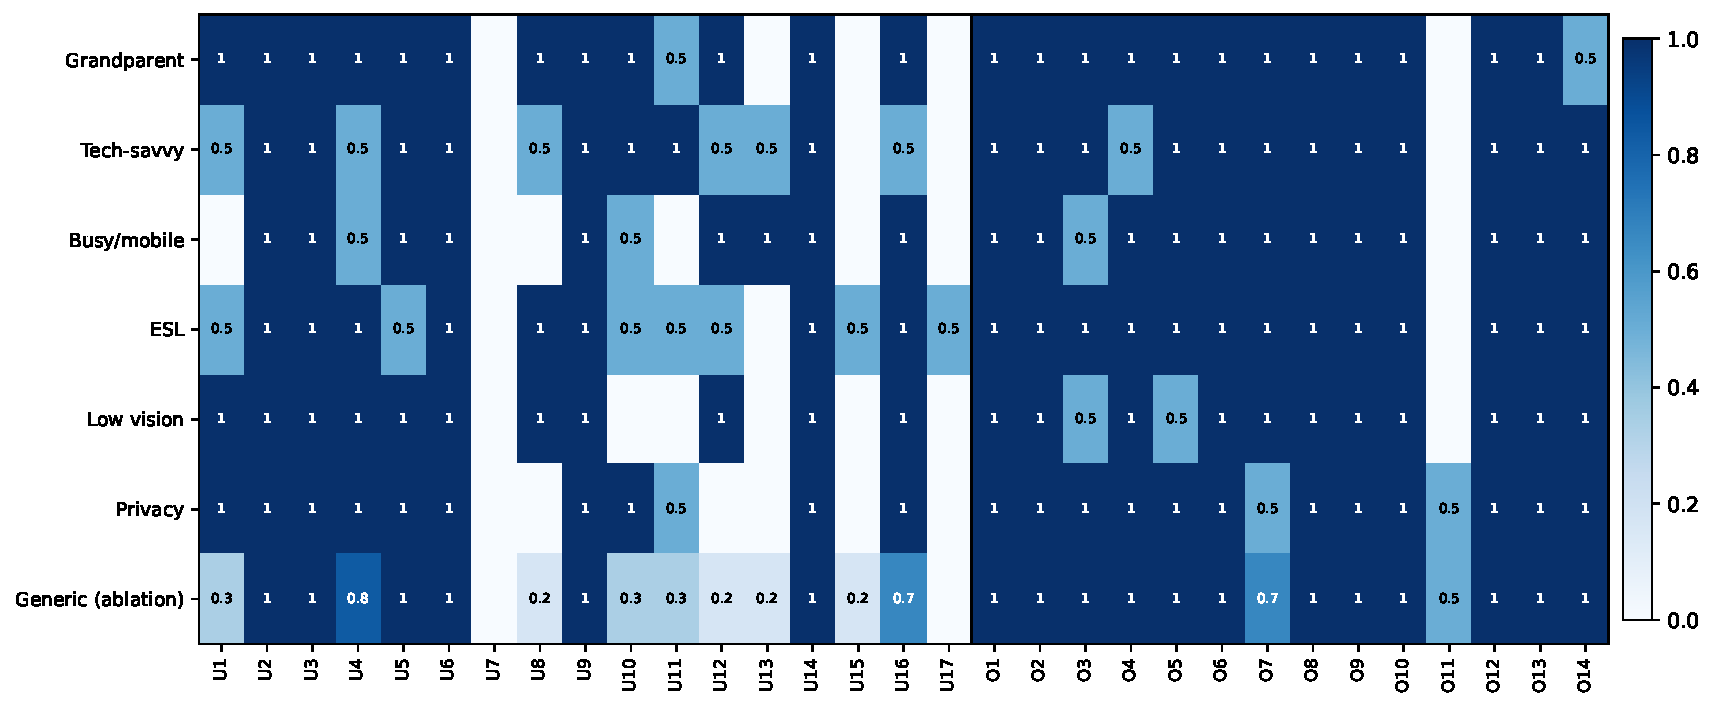
\includegraphics[width=\textwidth]{generated/figures/heatmap.pdf}
\caption{Detection rate of each seeded defect by persona (share of that persona's sessions whose findings matched the defect; two sessions per persona, six for the generic agent). Usability defects U1--U17 on the left, output defects O1--O14 on the right.}
\label{fig:heatmap}
\end{figure*}

\subsection{Does the persona matter?}
\label{sec:persona}

Figure~\ref{fig:heatmap} shows where personas differ. The 20$\times$20\,px icon-only page-turn buttons (U12) were reported in every session of the grandparent, the low-vision senior and the phone user, but in no session of the privacy-conscious parent and in one of six generic sessions. The child-photo upload without privacy information (U10) was reported by every session of the privacy-conscious parent, the grandparent (a privacy ``pragmatist'') and the tech-savvy parent, who calls a child's photo ``biometric-adjacent personal data''. The low-vision senior (``unconcerned-to-pragmatist'') never reported it, and the generic agent did in two of six sessions. The vague ``Proceed~$\to$'' button (U1) was reported by every session of the grandparent, the low-vision senior and the privacy-conscious parent, but by no session of the phone user, who acts on the first cue. The phone user reported in both sessions that a single page cannot be fixed without paying to regenerate the whole book (U13), which only one other persona session and one generic session reported. Only the parent reading English as a second language noticed the switch from dollars to pounds (U17), in one of her two sessions: ``I do not know if the currency changed because I am in England, or if the price was converted.'' These defects were on screen in every session, so these differences come from what the personas chose to report, not from what they happened to see.

The silent truncation (U8) is different. Every session in which a field kept fewer characters than were typed reported it (7 of 7 persona sessions, 1 of 1 generic session), but that happened in 7 of 12 persona sessions and only 1 of 6 generic sessions. The personas' memories are longer (120--220 characters, against 57 for the generic user), and personas tend to elaborate. The persona effect on U8 is therefore one of exposure, which the exposure-adjusted recall removes.

The persona also shapes \emph{which} defects are found. Two sessions of the same persona found more similar sets of usability defects (Jaccard \JacSame{}) than sessions of different personas (\JacCross{}; generic pairs \JacGeneric{}). The label-permutation test puts the difference of \LabelStat{} at $p \LabelP$. All three means lie above the range of 5--65\% that \citet{hertzum2001evaluator} report for the same any-two agreement measure between human evaluators. The comparison is loose, because our universe is 17 seeded, mostly conspicuous defects, but it suggests that simulated evaluators are more alike than people are, and that persona conditioning restores only part of the diversity.

\begin{figure}[t]
\centering
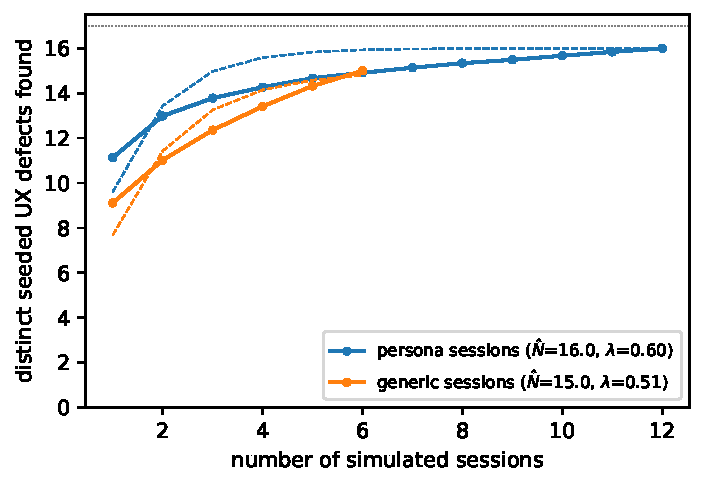
\includegraphics[width=\columnwidth]{generated/figures/discovery.pdf}
\caption{Distinct seeded usability defects found by $n$ sessions (mean over 500 random orders; dashed: Nielsen--Landauer fits; dotted: the 17 seeded defects).}
\label{fig:discovery}
\end{figure}

\subsection{Coverage and discovery}
\label{sec:coverage}

Together the persona sessions found \UnionUX{} of the 17 usability defects and all \UnionOut{} output defects (Figure~\ref{fig:discovery}). No session found the wizard's missing progress indicator (\NeverFound{}), an absence rather than something on screen, which a step-by-step agent that reviews one screen at a time rarely remarks on. \PersonaOnly{} (the currency switch) was found only by personas, and the generic sessions found \GenericOnly{} that the personas missed. With the ceiling free, the Nielsen--Landauer fit gives $\hat N=\NHat{}$ and $\lambda=\LambdaFree{}$ for personas (RMSE \RmseFree{}); fixing $N=17$ gives $\lambda=\LambdaSeeded{}$ (RMSE \RmseSeeded{}). For generic sessions, $\hat N=\NHatGeneric{}$ and $\lambda=\LambdaFreeGeneric{}$. These values are well above the average of $0.31$ for human participants~\cite{nielsen1993mathematical}, as expected for a benchmark of conspicuous seeded defects, and they should not be read as evidence that simulated sessions find more real problems than people.

At a matched budget, sessions drawn from \emph{different} personas found more distinct usability defects than the same number of generic sessions: \MatchedPersonaA{} vs \MatchedGenericA{} with one session, \MatchedPersonaB{} vs \MatchedGenericB{} with two and \MatchedPersonaC{} vs \MatchedGenericC{} with three. With six sessions both reached \MatchedPersonaF{}. Persona diversity therefore pays off when the budget is small; with enough sessions the generic agent catches up on this benchmark.

\begin{table}[t]
\centering
\small
\caption{Share of sessions in which each seeded output defect was reported by the persona-grounded output assessment versus flagged by the deterministic text metrics alone.}
\label{tab:output}
\begin{tabularx}{\columnwidth}{@{}l>{\raggedright\arraybackslash}Xcc@{}}
\toprule
ID & Seeded output defect & \begin{tabular}[b]{@{}c@{}}Output\\critic\end{tabular} & \begin{tabular}[b]{@{}c@{}}Metrics\\only\end{tabular} \\
\midrule
O1 & Typo in the book title & 1.00 & 0.00 \\
O2 & Unfilled template placeholders in dedication & 1.00 & 1.00 \\
O3 & Child's name misspelled on one page & 0.89 & 1.00 \\
O4 & Pronoun switch for the hero & 0.94 & 0.00 \\
O5 & The user's second character never appears & 0.94 & 0.89 \\
O6 & Invented character `Uncle Bartholomew' & 1.00 & 1.00 \\
O7 & Special object replaced by `a shiny red balloon' & 0.83 & 0.00 \\
O8 & Age-inappropriate vocabulary & 1.00 & 1.00 \\
O9 & Frightening passage for young children & 1.00 & 0.00 \\
O10 & Illustration contradicts text (rain vs. sunshine) & 1.00 & 0.00 \\
O11 & Hero's hair colour changes & 0.22 & 0.00 \\
O12 & Opening sentence repeated near the end & 1.00 & 1.00 \\
O13 & Final sentence cut off & 1.00 & 0.94 \\
O14 & Wrong illustration style & 0.94 & 0.00 \\
\bottomrule
\end{tabularx}
\end{table}


\subsection{Output critique}
\label{sec:outputresults}

Every output defect was found by at least one session, and twelve of the fourteen in at least 89\% of sessions (Table~\ref{tab:output}). Every session recognised the title typo, the unfilled placeholders, the invented uncle, the ornate vocabulary, the frightening passage, the sunshine illustration under pouring rain, the repeated opening and the truncated ending. The hardest defect was the hero's hair-colour change on one page (O11), found in 22\% of sessions. It requires comparing pictures across pages, which the critic reviews as separate parts. Personas and the generic agent differed little on output. The generic agent found O11 more often (3 of 6 sessions against 1 of 12), whereas personas more often noticed that the treasured object had become a red balloon (O7; 11 of 12 against 4 of 6).

The deterministic text metrics alone flag \DetBaseline{} of the 14 output defects on average. They catch placeholders, near-miss names, the missing and the invented character, the reading level, the repetition and the truncated ending. They miss the title typo, because the typo check only reads sentence-like lines, and they have no rule at all for the pronoun switch, the object swap, the frightening content, the style or anything in the pictures. The LLM critique is thus doing most of the work, with the metrics serving as checkable evidence. Beyond detection, every part receives a change and usually a rewrite. On the page where the uncle appears, the grandparent's critic flagged the invented character and the pronoun switch (``she followed him''), and proposed: ``Grandma Maggie came up the path carrying a basket. `Hold the kite high,' she said. `Let the wind lift it!'\,'' (Appendix~\ref{app:example}).

\begin{table}[t]
\centering
\small
\caption{Paired vision ablation: share of the 14 sessions in which the re-run output assessment reported each seeded output defect when it could see the pictures versus text and alt text only (same captured outputs).}
\label{tab:vision}
\begin{tabularx}{\columnwidth}{@{}l>{\raggedright\arraybackslash}Xcc@{}}
\toprule
ID & Seeded output defect & \begin{tabular}[b]{@{}c@{}}With\\pictures\end{tabular} & \begin{tabular}[b]{@{}c@{}}Text and\\alt text\end{tabular} \\
\midrule
O1 & Typo in the book title & 1.00 & 1.00 \\
O2 & Unfilled template placeholders in dedication & 1.00 & 1.00 \\
O3 & Child's name misspelled on one page & 1.00 & 1.00 \\
O4 & Pronoun switch for the hero & 0.93 & 0.93 \\
O5 & The user's second character never appears & 0.93 & 0.79 \\
O6 & Invented character `Uncle Bartholomew' & 1.00 & 1.00 \\
O7 & Special object replaced by `a shiny red balloon' & 1.00 & 0.93 \\
O8 & Age-inappropriate vocabulary & 0.93 & 1.00 \\
O9 & Frightening passage for young children & 1.00 & 1.00 \\
O10 & Illustration contradicts text (rain vs. sunshine) & 1.00 & 0.00 \\
O11 & Hero's hair colour changes & 0.21 & 0.00 \\
O12 & Opening sentence repeated near the end & 1.00 & 1.00 \\
O13 & Final sentence cut off & 1.00 & 1.00 \\
O14 & Wrong illustration style & 0.86 & 0.86 \\
\bottomrule
\end{tabularx}
\end{table}


\subsection{Vision ablation}
\label{sec:vision}

On identical captures, taking the pictures away removed every detection of the picture-only defects (Table~\ref{tab:vision}): \VisVisualMean{} with pictures against \NoVisVisualMean{} with text and alt text (McNemar: \McBVisual{} session--defect pairs detected only with pictures, \McCVisual{} only without, $p \McPVisual$; better with pictures in \SignWVisual{} of \AblRuns{} sessions). For the textual defects, the difference was negligible (\VisTextualMean{} vs \NoVisTextualMean{}; \McBTextual{} vs \McCTextual{} discordant pairs, $p \McPTextual$). Across all output defects, recall was \VisAllOutMean{} with pictures and \NoVisAllOutMean{} without ($p \McPAllOut$; better in \SignWAllOut{} sessions, worse in \SignLAllOut{}). The alt text never said that it was sunny or that the hair had changed, so a critic without pictures could not know; an output critic for illustrated products must see the illustrations.

\subsection{Reliability and precision}
\label{sec:reliability}

The judge and the keyword baseline agreed on \AgreeJK{} of session--defect decisions ($\kappa=\KappaJK{}$, substantial). Repeating the output assessment on the same captures gave \RetestAgree{} agreement on which output defects were found ($\kappa=\RetestKappa{}$, moderate), with the same recall (\RetestRecallAMean{} and \RetestRecallBMean{}). Kappa is only moderate despite the high agreement because most defects are found in nearly every session, which leaves little room above chance. Half of the 12 disagreements concern the hair-colour change (O11); the rest are spread over four defects. The in-session assessment and a re-run with the later assessor version agreed on \OrigRerunAgree{} ($\kappa=\OrigRerunKappa{}$).

Pooled over sessions, the \PooledFindings{} findings comprise \PooledMatched{} first matches, \PooledDuplicate{} duplicates, \PooledUnseeded{} valid but unseeded findings (\UnseededShare{}) and \PooledIncorrect{} incorrect ones. In the audit sample of \AuditN{} valid-unseeded findings, \AuditValid{} were valid (\AuditValidPct{}, 95\% CI \AuditValidCI{}), and \AuditOverlap{} of these in fact described seeded defects that the strict judge had not matched; \AuditDebatable{} were debatable and \AuditWrong{} wrong or partly wrong. Correcting the lenient precision with the audit gives \AdjPLenient{} (CI \AdjPLenientCI{}). The wrong findings were a hallucinated typo, a checkout problem filed as missing book content, a claim that the cover lacks a rocking horse it shows, and a complaint that blamed the site for the persona's own phrase ``Grandpa's old blue shirt'', the E1 failure of \S\ref{sec:errors}.

\begin{table*}[t]
\centering
\footnotesize
\setlength{\tabcolsep}{3.5pt}
\caption{Post-session self-report by persona (mean $\pm$ SD): SUS (0--100), UEQ-S pragmatic/hedonic ($-3$..$3$), likelihood to recommend (0--10), keepsake-worthiness of the generated book (1--5), mean in-session valence ($-2$..$2$), SUS acquiescence-consistency flags, and the persona-fidelity audit (1--5; lower caricature/leakage is better).}
\label{tab:questionnaires}
\begin{tabular}{lcccccccccc}
\toprule
Persona & SUS & \begin{tabular}[b]{@{}c@{}}UEQ-S\\pragmatic\end{tabular} & \begin{tabular}[b]{@{}c@{}}UEQ-S\\hedonic\end{tabular} & Recommend & Keepsake & Valence & \begin{tabular}[b]{@{}c@{}}SUS\\flag\end{tabular} & Realism & Caricature & Leakage \\
\midrule
Grandparent & 37.5 $\pm$ 10.6 & 0.12 $\pm$ 0.18 & $-$0.50 $\pm$ 0.00 & 1.5 $\pm$ 0.7 & 1.0 $\pm$ 0.0 & 0.27 $\pm$ 0.13 & 0/2 & 4.0 $\pm$ 0.0 & 2.0 $\pm$ 0.0 & 1.5 $\pm$ 0.7 \\
Tech-savvy & 38.8 $\pm$ 12.4 & 1.00 $\pm$ 0.71 & $-$0.38 $\pm$ 0.53 & 0.0 $\pm$ 0.0 & 1.0 $\pm$ 0.0 & $-$0.45 $\pm$ 0.42 & 1/2 & 4.5 $\pm$ 0.7 & 2.0 $\pm$ 0.0 & 1.0 $\pm$ 0.0 \\
Busy/mobile & 48.8 $\pm$ 5.3 & $-$0.62 $\pm$ 0.53 & 0.62 $\pm$ 0.53 & 1.5 $\pm$ 0.7 & 1.0 $\pm$ 0.0 & 0.42 $\pm$ 0.00 & 0/2 & 5.0 $\pm$ 0.0 & 2.0 $\pm$ 0.0 & 1.0 $\pm$ 0.0 \\
ESL & 21.2 $\pm$ 1.8 & 0.88 $\pm$ 0.18 & 0.12 $\pm$ 1.24 & 0.0 $\pm$ 0.0 & 1.0 $\pm$ 0.0 & $-$0.15 $\pm$ 0.04 & 0/2 & 5.0 $\pm$ 0.0 & 1.5 $\pm$ 0.7 & 1.0 $\pm$ 0.0 \\
Low vision & 38.8 $\pm$ 8.8 & $-$0.75 $\pm$ 0.35 & 0.00 $\pm$ 0.71 & 2.5 $\pm$ 0.7 & 1.0 $\pm$ 0.0 & 0.47 $\pm$ 0.21 & 1/2 & 4.0 $\pm$ 0.0 & 2.5 $\pm$ 0.7 & 1.5 $\pm$ 0.7 \\
Privacy & 40.0 $\pm$ 17.7 & $-$1.00 $\pm$ 0.71 & 0.00 $\pm$ 0.00 & 1.0 $\pm$ 0.0 & 1.0 $\pm$ 0.0 & $-$0.29 $\pm$ 0.21 & 1/2 & 4.5 $\pm$ 0.7 & 2.0 $\pm$ 0.0 & 1.5 $\pm$ 0.7 \\
Generic (ablation) & 42.5 $\pm$ 10.0 & $-$0.88 $\pm$ 0.56 & 0.42 $\pm$ 0.54 & 0.5 $\pm$ 0.5 & 1.0 $\pm$ 0.0 & 0.26 $\pm$ 0.19 & 4/6 & -- & -- & -- \\
\bottomrule
\end{tabular}
\end{table*}


\subsection{Self-report and fidelity}
\label{sec:selfreport}

\site{} is deliberately bad, and every persona gave it a failing SUS score (Table~\ref{tab:questionnaires}). The parent reading English at B1 scored it lowest (\SusEslParent{}), consistent with the jargon, the Lexile codes and the cryptic error, and the phone user scored it highest (\SusBusyParentMobile{}). Every session rated the book 1 of 5 as a keepsake. The generic agent gave inconsistent answers to paired positive and negative SUS items in 4 of 6 sessions, against 3 of 12 persona sessions, which is one more reason to distrust simulated questionnaires~\cite{tjuatja2024llms,dominguez2024questioning}. In-session valence (Figure~\ref{fig:valence}) follows the journey: positive on the home page and the log-in form, a dip at the dashboard with its cryptic error banner (step 3), recovery in the wizard, then a fall at the book and the checkout. Averaged over all steps on a page, valence was $-0.65$ on the dashboard, $-1.13$ on the book and $-0.56$ at the checkout, against $+0.82$ in the wizard. In one session, the privacy-conscious parent recorded that she would abandon at the privacy notice (step 5), which is too vague ``to share sensitive information about my child''; the other five self-reported abandonments were all at the checkout. Per-persona means of the fidelity audit were 4.0--5.0 for realism, 1.5--2.5 for caricature and 1.0--1.5 for knowledge leakage. The audit uses the same model as the agent, and we read these ratings as a screen for gross failures, not as validation.

\begin{figure}[t]
\centering
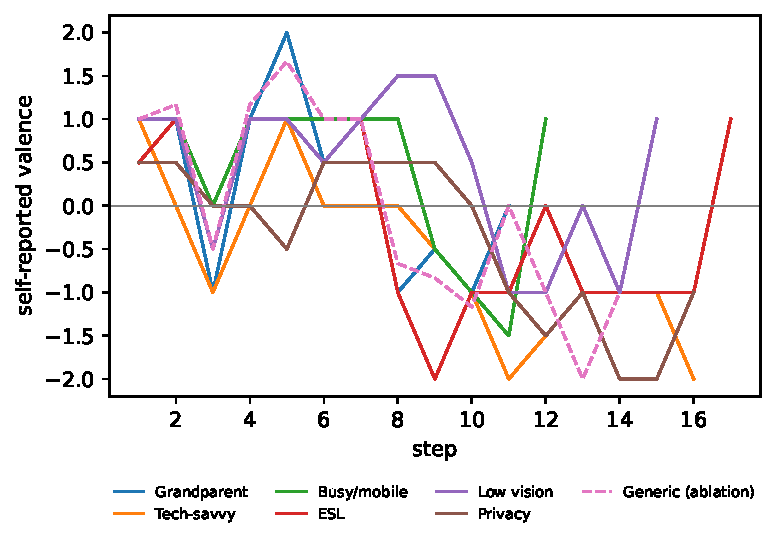
\includegraphics[width=\columnwidth]{generated/figures/valence.pdf}
\caption{Mean self-reported valence by step and persona (\site{}).}
\label{fig:valence}
\end{figure}

\section{Case study: ourlegacy.family}
\label{sec:case}

\ol{} is a live product that turns a family story into an illustrated book, with a PDF export and a printed hardcover. We ran the grandparent persona, Margaret, 71, a retired Year~2 teacher whose father made her a kite from an old blue shirt, and who wants a book for her grandson Oliver.

\paragraph{First attempt.} The first session stopped after eight steps. At step 5, the agent ticked the site's ``Verify you are human'' check, waited 60\,s for a change that never came, and then clicked a control that had vanished. This led to the security-check reflex of \S\ref{sec:env} and to launching Chrome with the persona's locale.

\paragraph{Session B: creating the book.} In the second session (16 steps, 21 LLM calls, 505\,s including the post-session stages), the check passed on the first tick in 1.0\,s. Margaret signed up with a disposable inbox and entered the one-time code it received. She declined to upload a photograph of her grandson, typed her memory, and paid for the book from the new account's free credits. After waiting 9, 75 and 21\,s for the generation, she read all ten scenes. Her issue reports included ``The story has changed the family relationships incorrectly'' (severity 4, quoting ``One summer, Grandpa's daddy made something very special'' and ``Now Grandpa was old --- and he had a grandson of his own''). The product had made the storyteller a grandfather and her father ``Grandpa's daddy''. Her own wording may have contributed: her memory includes the sentence ``I help him fly Grandpa's blue kite'', using her persona's name for the kite. But it also calls Oliver ``my grandson'', and her character card describes ``Grandma Maggie, Oliver's grandmother''. The output review of 11 parts, as re-run after the fixes of \S\ref{sec:errors}, scored fidelity and character consistency 1 of 5 and quoted her input against the output: ``My input said, `My father taught me how to hold the string\ldots' The output says `Grandpa's daddy showed him,' changing me into him.'' She gave the site a SUS of 60 and the book 2 of 5 as a keepsake.

\paragraph{Session C: returning to repair it.} The third session was a return visit (30 steps, 40 calls, 1,007\,s). Margaret was given her memory of the first visit and asked to open the same book, try the site's editing tools and export the PDF. She rewrote the text of the first two scenes and asked for their pictures to be redrawn so that they showed her as a little girl, once for the first scene and twice for the second. She then personalised the export (title ``The Blue Kite'', author, dedication, ``This book belongs to Oliver Ellison'') and generated a 32-page PDF. She also slipped, as a person might: she typed ``5'' into ``Teller's age''. When the PDF's title page read ``told by Margaret Ellison, age 5'', she cleared the field and regenerated the PDF. The issue she reported at that point is a useful kind of finding. It blames the field label rather than herself (``Clarify the field as `Age of the person telling the story'\,''). The assessor critiqued 47 parts of the final versions, after superseding 52 earlier captures. It found that the site's tools could fix the first scenes but that the later ones still said ``Grandpa's daddy'' and showed an elderly man where Margaret should be. Margaret gave a SUS of 25 and the book 1 of 5: ``The website made a pretty book with a lovely blue kite, but it did not yet make my family's story true, so I would not give it to Oliver.''

\begin{table*}[t]
\centering
\footnotesize
\caption{Five failure modes of the evaluator found in the \ol{} sessions (B: creating the book; C: the return visit). Each was fixed and the stage re-run on the recorded session. ``Before'' and ``after'' quote the evaluator; ``after'' is the last re-run of the stage, and the E3 ``before'' is the in-session assessment, recovered from the LLM call log.}
\label{tab:errors}
\begin{tabularx}{\textwidth}{@{}P{2.1cm}YYP{3.6cm}Y@{}}
\toprule
Failure mode & Before & Cause & Fix & After \\
\midrule
E1 Wording provenance (B) & ``The title says `Grandpa's Blue Kite,' although the kite was made by my father\ldots'' and a proposal to rename the book & The site built the title from Margaret's own phrase ``I help him fly Grandpa's blue kite''; the critic could not tell her words from the site's & List the wording the output shares with the user's inputs as ``came from you''; check inputs before blaming the site & ``The title is fine as a name for the kite, but the story has silently changed Margaret into a male narrator called Grandpa.'' \\
\addlinespace
E2 Edit history (C) & ``The teller age changed from 5 to Optional''; top change: ``preserve the teller age of 5'' & Inputs were listed by label only; a cleared field and a later correction looked like the site's changes, and the edit boxes of different scenes (all ``Narrative Text'') were conflated & Record step, screen and element per input; mark replaced and cleared entries & ``The site correctly retained my decision to clear the teller's age and now shows `Optional.'\,'' \\
\addlinespace
E3 Version confusion (C) & 63 parts from 88 captures; ``The narrator was incorrectly labeled as five years old in the first preview''; top change: ``Correct the narrator metadata and all age statements so I am not described as five years old'' & Captures of the same page or file at different times were reviewed as separate parts & Supersede by prose overlap and regenerated-file matching; attach change notes & 47 parts; 52 captures superseded, 34 change notes, e.g.\ ``no longer there: `As told by Margaret Ellison, age 5 \ldots'\,'' \\
\addlinespace
E4 Cross-visit provenance (C) & Invented, in a re-run without the earlier-visit inputs: ``A physical Wales visit involving Oliver and Grandpa'', ``The green wellies and specific present-day trip details'', ``A repeated family tradition of flying the kite in Wales'' & Only the current visit's inputs were shown; these details were in the story Margaret typed on her first visit & Carry the inputs of earlier visits forward, tagged, with element identity scoped per visit & Used correctly: ``Oliver's brown curly hair, freckles and green wellies''; changed: ``The original `today' visit is changed into an invented `next day' trip back to Wales'' \\
\addlinespace
E5 Missing environment events (C) & Knowledge leakage 3: ``claims complete inspection of a 32-page PDF immediately after page navigation failed, which exceeds what the recorded actions support''; realism 3 & The audit transcript omitted what the browser reported, here that it had opened the downloaded PDF and paged through it & Put each step's events into the transcript before the thought & Two audits: leakage 1 and realism 4 in both; one still notes a ``continuity problem'' at that step \\
\bottomrule
\end{tabularx}
\end{table*}

\subsection{Failure modes of the evaluator}
\label{sec:errors}

Reading the \ol{} reports critically revealed five failure modes of the evaluator (Table~\ref{tab:errors}). All five are \emph{attribution} errors: the evaluator was right about what it saw, but wrong about who had caused it or what had happened. E4 and E5 cannot arise on \site{}, which is visited once and produces no browser events. E2 and E3 rarely can, because the persona enters its story once and never edits it or regenerates the book. E1 can, and did: the grandparent's own phrase ``Grandpa's old blue shirt'' caused one of the four wrong findings in the audit sample (\S\ref{sec:reliability}). The live site's editing tools, regenerated PDFs and repeat visits exposed the rest. They matter for any evaluator of generative products, because they turn the user's own words, edits and earlier choices into accusations against the site.

The fixes interact. Once the critic checked its inputs carefully (E1), it began to flag details that Margaret had entered on her \emph{first} visit as inventions (E4). We reproduced E4 by re-running the final assessment without the earlier-visit inputs, and the invented list returned. Table~\ref{tab:errors} quotes this re-run, because the intermediate assessment in which we first saw the problem was not kept. For E5 we checked the change against run-to-run variation. Both audits of the event-free transcript (the original and a repeat) complained that Margaret claimed to have seen all 32 pages after page navigation failed, and both scored realism 3. With the events in the transcript, two audits scored realism 4 and leakage 1, and only one mentioned the step, as a ``continuity problem''. That is a fair point about the environment, which reads a file in one step where a person would page through it. Repeated audits of an unchanged transcript varied by one point on some scales, so single audit scores should be read with that resolution in mind.

\subsection{Cost}

The two complete sessions cost nothing in API fees; the model is free. They used 61 LLM calls, about 0.6\,M tokens, and 25 minutes of wall time. The site's free starter credits paid for the book and the redrawn pictures. The re-runs for the fixes above needed no new browsing.

\section{Discussion}
\label{sec:discussion}

\paragraph{What the persona buys.} Persona conditioning raised usability recall by about ten percentage points and made sessions of the same persona more alike than sessions of different personas. The differences are the ones a usability researcher would predict from the personas. They appear exactly where persona attributes should matter: small targets for the low-vision and phone users, photo privacy for the privacy-minded, currency for the second-language reader. The price is lower strict precision, and the benefit shrinks as the number of sessions grows. We read this as supporting personas as a way to diversify a small budget of simulated sessions, not as evidence that simulated users are faithful stand-ins for these groups.

\paragraph{Reading the output.} For generative products, output critique is where most of the value lies. The critic found every seeded output defect, proposed concrete changes and rewrites, and on the live site it identified the product's central failure: the book told the family's story with the wrong people in it. Two design lessons stand out. First, a critic of illustrated output must see the pictures. Second, attribution is the hard part, not detection. Every evaluator failure we found on the live site was an attribution error, and each required recording more of the session: the order and target of inputs, the version history of outputs, earlier visits, and what the environment itself did.

\subsection{Limitations}
\label{sec:limitations}

\begin{itemize}
\item \textbf{One synthetic benchmark.} \site{} was built by us, its defects are conspicuous, and the people who seeded them know what LLMs notice. Recall on real sites with real, subtler problems is unknown; the \ol{} study is qualitative.
\item \textbf{No human scoring.} The judge is the same model as the agent, and the audit sample was labelled by the AI coding assistant that built \site{}, not by a person. The keyword baseline, the audit and $\kappa$ with the baseline mitigate but do not replace independent human annotation, which is the most important next step.
\item \textbf{Code versions.} The \site{} numbers come from versions of the assessor that predate the attribution fixes (\S\ref{sec:setup}). Re-running the \site{} output assessments with the final code would show whether the fixes change recall or precision there.
\item \textbf{Small samples and one model.} We ran two sessions per persona and six generic sessions, with one model and one temperature. The $p$-values are nominal. The model is a ``stealth'' model that may be withdrawn, so sessions cannot be replayed with it, although every call is logged and every score can be recomputed.
\item \textbf{Confounds.} Persona sessions were longer, and the generic user's facts were shorter, which affected exposure to the truncation defect. Exposure adjustment addresses the latter but not the former.
\item \textbf{Assumptions in the environment.} Perception notes (``some controls are tiny''), the truncation notice, the security-check reflex and the automatic reading of files encode our assumptions about what people perceive and do. They help detection (U8, U12), and they may overstate what real users notice.
\item \textbf{Persona validity.} We audited fidelity with an LLM. We did not compare the simulated users with real people from these groups, and plausible-sounding behaviour is not evidence of realistic behaviour~\cite{wang2025large,agnew2024illusion}.
\end{itemize}

\subsection{Ethics and responsible use}

Simulated users do not replace studies with people, least of all with older adults, people with disabilities or second-language readers, whose experience a model can caricature or flatten~\cite{cheng2023compost,wang2025large,agnew2024illusion}. We see \sys{} as a pre-screening and regression tool: it finds conspicuous problems cheaply before a study, and keeps checking outputs after changes. It should run only on sites one owns or is allowed to test. Our live runs used small budgets, a disposable inbox and a new account's free credits, and never paid or entered payment details. Ticking a ``verify you are human'' box is what a person does, but automating it on sites that have not agreed to testing may breach their terms; the reflex never solves image or puzzle challenges and should not be used to get around bot protection. The personas' family stories are fictional, and logs are redacted of tokens and one-time codes.

\paragraph{Use of AI assistance.} An AI coding assistant wrote most of \sys{} and \site{}, ran the experiments, labelled the audit sample and drafted this paper. The \site{} results are generated by the analysis script from the committed run records, and the case-study figures are taken from the committed run summaries.

\section{Conclusion}
\label{sec:conclusion}

We built and evaluated a persona-grounded agent that evaluates both a website's usability and everything the website generates. On a benchmark with 31 seeded defects, persona conditioning raised usability recall and diversified what was found, pictures were essential for critiquing illustrations, and the output critic found every seeded output defect in at least one session. On a live product, the agent documented a serious fidelity failure that a usability-only evaluation would miss. Our analysis of its own mistakes points to the central open problem for evaluating generative products: deciding correctly who made each part of what the user sees.

\bibliographystyle{plainnat}
\bibliography{refs}

\appendix
\onecolumn

\section{Personas}
\label{app:personas}

\begin{table}[h]
\centering
\footnotesize
\caption{The persona library used in the experiments (abbreviated). Facets: motivation / information processing / computer self-efficacy / risk attitude / learning style. Every persona also has a backstory, goals, frustrations, Big Five descriptors and family facts; the generic baseline keeps only the family facts.}
\label{tab:personas}
\begin{tabularx}{\textwidth}{@{}P{3.1cm}P{1.9cm}YYP{2.2cm}@{}}
\toprule
Persona & Device, attention, patience & Facets & Attitudes, language, accessibility & Story facts \\
\midrule
Margaret Ellison (71), retired primary-school teacher & desktop, full, 7 & task-focused / comprehensive / low / risk-averse / process-oriented & privacy pragmatist; price sensitivity medium-high; trust in AI low-medium; native English; mild presbyopia & Oliver (5), Grandma Maggie, a blue kite \\
\addlinespace[3pt]
Daniel Okafor (41), backend engineer & desktop, full, 8 & tech-curious / selective / high / risk-tolerant / tinkering & pragmatist leaning fundamentalist about his child's data; price sensitivity low; knows AI failure modes & Zara (7), Dad, a purple sock flag \\
\addlinespace[3pt]
Priya Nair (36), A\&E nurse on shifts & phone, skim, 4 & task-focused / selective / medium / risk-averse / process-oriented & pragmatist; price sensitivity high; time pressure very high & Aarav (5), Meera, a toy dinosaur \\
\addlinespace[3pt]
Minh Tran (33), pastry chef & desktop, full, 6 & task-focused / comprehensive / medium / risk-averse / process-oriented & English CEFR B1, first language Vietnamese; price sensitivity high & Linh (4), Bà Nội, a paper lantern \\
\addlinespace[3pt]
Harold Brooks (78), retired carpenter & 200\% zoom, low vision, 8 & task-focused / comprehensive / low / risk-averse / process-oriented & macular degeneration; cannot read low-contrast or small text; struggles with small and icon-only controls; privacy unconcerned-to-pragmatist & Lily (4), Grandpa Harold, a rocking horse \\
\addlinespace[3pt]
Elena Petrova (45), paralegal & desktop, full, 6 & task-focused / comprehensive / medium / risk-averse / process-oriented & privacy fundamentalist (Westin); trust in AI low; fluent English (native Bulgarian) & Nikolai (6), Mama, a ``brave stone'' \\
\addlinespace[3pt]
Generic user (baseline) & desktop, full, 6 & --- (no persona conditioning) & --- & Sam (5), Grandpa Joe, a yellow bucket \\
\bottomrule
\end{tabularx}
\end{table}

\section{Seeded usability defects}
\label{app:defects}

\begin{table}[h]
\centering
\footnotesize
\caption{The 17 usability defects seeded into \site{}, with the page and the heuristic or code they violate.}
\label{tab:uxdefects}
\begin{tabularx}{\textwidth}{@{}lllY@{}}
\toprule
ID & Page & Code & Defect \\
\midrule
U1 & home & H2/H4 & The main call to action is labelled ``Proceed~$\to$'' instead of saying what it does \\
U2 & home & H2 & Jargon value proposition (``Leverage our multimodal generative narrative engine to synthesise bespoke, heirloom-grade story artefacts\ldots'') \\
U3 & all & ACC & Footer links (privacy, terms, contact) at about 1.4:1 contrast \\
U4 & home & ACC & Hero illustration without alt text \\
U5 & log-in & H6/ACC & Placeholder-only labels that disappear when typing \\
U6 & dashboard & H9 & ``Error 0x80070057: profile sync incomplete'' with no explanation or action \\
U7 & wizard & H1 & The four-step wizard never shows which step you are on or how many remain \\
U8 & wizard & H5/H1 & The memory textarea silently truncates at 200 characters \\
U9 & wizard & H2 & Reading levels given as Lexile codes (``BR--200L'') instead of ages \\
U10 & wizard & TRUST & Asks for a clear photo of the child's face without saying how it is stored, used or deleted \\
U11 & wizard & H1 & 15-second generation with an unlabelled spinner \\
U12 & book & ACC/H6 & 20$\times$20\,px icon-only page-turn buttons without accessible names \\
U13 & book & H3 & The only way to change anything is ``Regenerate entire book -- \$4.99'' \\
U14 & checkout & DECEPTIVE & ``Premium gift wrap \pounds7.99'' ticked by default \\
U15 & checkout & DECEPTIVE/VALUE & \pounds12.99 shipping appears only at checkout \\
U16 & checkout & DECEPTIVE & ``Your price is reserved for 09:59'' countdown \\
U17 & checkout & H4/VALUE & Prices quoted in dollars, checkout charged in pounds \\
\bottomrule
\end{tabularx}
\end{table}

\section{Example output critique}
\label{app:example}

Two parts from the grandparent's first \site{} session, verbatim except for layout. The book's hero is Oliver; the family memory is about flying a blue kite with Grandma Maggie on a windy hill in Wales.

\medskip
\noindent\textbf{Page 4.} \emph{Text:} ``Suddenly, Uncle Bartholomew appeared with a lantern. `Oliver, follow me!' he called, and she followed him along the winding path.'' \emph{Picture:} ``A tall dark-haired figure labeled `Uncle Bartholomew' stands beside Oliver on the hill near the farmhouse, holding a small yellow lantern.'' \emph{Reaction:} ``This page introduces an unexpected stranger and then changes Oliver's pronoun from he to she, which is a serious error.'' \emph{Problems:} fidelity, severity 3 (``Uncle Bartholomew is not in the supplied family story''); language, 4 (``she followed him'' after he/him pronouns); coherence, 4 (he appears ``with no setup or explanation''); text--image fit, 2 (the winding path is not shown). \emph{Change:} ``Remove Bartholomew and the invented adventure, keep Oliver's pronouns consistent, and bring Grandma Maggie into the actual memory.'' \emph{Rewrite:} ``Grandma Maggie came up the path carrying a basket. `Hold the kite high,' she said. `Let the wind lift it!' Oliver smiled and ran with her to the top of the hill.''

\medskip
\noindent\textbf{Page 5.} \emph{Text:} ``Deep in the woods, the shadows grew teeth and whispered that no one would ever find Oliver again. Oliver clutched a shiny red balloon and trembled in the dark.'' \emph{Reaction:} ``The threatening shadows and claim that no one would find Oliver are frightening for a five-year-old, and the red balloon has not been prepared.'' \emph{Problems:} age fit, 4; fidelity, 4 (``A red balloon, dark woods, and a threat are invented and displace the hill, farmhouse, kite, and family memory''); coherence, 4; text--image fit, 2. \emph{Change:} ``Replace the frightening scene with a safe, playful moment on the Welsh hill involving the kite and Grandma Maggie.'' \emph{Rewrite:} ``The kite dipped toward the grass. Oliver gave it a gentle pull, and it climbed high again. `I can feel the wind!' he laughed. Grandma Maggie stood beside him and cheered.''

\medskip
\noindent\textbf{Top changes (global).} ``Repair the entire story before checkout: complete the ending, remove the duplicate `The End,' fix `Adventrue,' replace `Olive,' and correct every pronoun and placeholder.'' ``Rewrite the plot around the actual memory: Oliver, Grandma Maggie, the Welsh hill, the old farmhouse, and the blue kite made from Grandpa's old blue shirt.'' \emph{Would pay:} ``no --- I would not pay \pounds45.97 for a preview with visible placeholders and spelling errors, an unfinished ending, and a story that does not preserve the memory I wanted to pass to Oliver.''

\section{Reproduction}
\label{app:repro}

The repository contains the code, the persona library, \site{} with its ground truth, and every session reported here. Screenshots and captured pictures are not committed, but all JSON records, traces, LLM call logs and captured output text are, so scoring and analysis reproduce every number without new LLM calls:

{\small
\begin{verbatim}
python experiments/score_ground_truth.py runs/suite/main          # cached judge decisions
python experiments/score_ground_truth.py runs/suite/main --variant vision   # also novision, vision2
python experiments/analyze.py --main runs/suite/main --out paper/generated
cd paper && tectonic main.tex
\end{verbatim}
}

\noindent New sessions and re-assessments need an OpenRouter key in a git-ignored \texttt{.env} file, and re-assessments with pictures also need the local screenshots:

{\small
\begin{verbatim}
python demo_sites/storyhearth/serve.py --port 8765 &
python experiments/run_suite.py --site storyhearth --name main --reps 2 --personas <ids>
python -m userqa reassess runs/suite/main/2026* --variant novision --no-vision
python -m userqa run --site ourlegacy --persona grandparent_storykeeper
python -m userqa run --site ourlegacy_revisit --persona grandparent_storykeeper --previous-run <run>
python -m userqa reaudit <run>
\end{verbatim}
}

\end{document}
